\documentclass[10pt]{jarticle}
\usepackage{float}
\usepackage{adrobo_abst}
\usepackage[dvipdfmx]{graphicx}
\usepackage{amssymb,amsmath}
\usepackage{bm}
\usepackage[superscript]{cite}
\usepackage{enumerate}
\usepackage{url}
%\usepackage[absolute]{textpos}

\renewcommand\citeform[1]{(#1)}

\begin{document}
    
    \makeatletter
    \doctype{2023年度卒業論文概要}
    \title{論文の作成について}{(副題がある場合は括弧でくくる)}
    \etitle{Making Research Paper}{($\bigcirc\bigcirc\bigcirc$)}
    
    \author{20C1119\hspace{.5zw}森田大雅}
    \eauthor{Hiromasa Morita}
    
    \makeatother
    
    \abstract{When preparing the manuscript, read and observe carefully this sample as well as the instruction manual for the manuscript of the Transaction of Japan Society of Mechanical Engineers. This sample was prepared using MS-word. Character size of the English title is 14 pts of Times New Roman as well as sub-title. The name is 12 pts. The address of the first author and the abstract is 10 pts of Times New Roman. Character spacing of the abstract is narrowed by 0.2 pts preferably.}
    
    \keywords{Mechanical Engineering, Keywords List}
    
    \maketitle
    
    \supervisor{指導教員:藤江真也 教授}
    
    \section{導\hspace{2zw}入}%===========================
	描画ロボットの研究において、シンプルにエッジ抽出を用いて人物画を描く研究[1]や、エッジ抽出とハッチングから芸術的な人物画を鉛筆で描く研究[2]、リモートユーザがタブレットを介してロボットに描かせる研究[3]などが存在する.
	これらの研究では模写や芸術的な表現が可能になっている.
	しかし、「人のような描き方」を追求したものが少ないと感じた.
	そこで、本研究ではウィリアム・ブーグローという画家が描いた「金髪女の横顔」という作品の画像を使い、できるだけ人が描いたような描き方をする描画ロボットと作成する.
	なお、人のような描き方とは描き順のことである.
	今回対象とする絵は頭部である.
	頭部を描く理由としては表情からこの絵に描いた様々な意味を連想させたり、本来は一場面の静止した場面にストーリーをもたらしたりする魅力がある.
	また、背景などの他の要素をより際立たさせることなどもできる.
	これは絵画以外に漫画などにも当てはまることで、それだけ頭部を描く重要性は高い.
	\\
	現代において鉛筆デッサンをする場合、線画を描く、つまり輪郭をはっきり描く方法は一般的ではない.
	これは古典的なデッサンの方法で昔の巨匠、例えばミケランジェロやダビンチなどが輪郭を描いている.
	しかし全く行われないというわけでもなく、画家によっては輪郭を描く.
	また、輪郭を描くことで何かしら特別な意味を込めたい場合などに描く場合もある.
	
    
    
    
    \section{システム構成}
	\subsection{Hardware}
	ハードウェアはAdeeptのADA031というマニピュレータキッドを用いている.
	Arduinoを用いて動作させるロボットであったため、OpenCVなどを使って簡単に画像の読み込みを行ったり、エッジ抽出をすることができなかった.
	そこで、基盤をRaspberry\ Piに代え、サーボモーターに接続するためにブレッドボードやジャンパー線、抵抗などを用いて少々改良を行っている.

	\subsection{Image Processing}
	先にも述べたが今回はウィリアム・ブーグローという画家の「金髪女の横顔」という絵の画像を用いる.
	選定理由は背景が白でシンプルであったため、画像を読み込む際にノイズが少なく綺麗にエッジ抽出を行えると考えたからである.
	この画像から
	前処理として任意の一枚の画像をガウシアンフィルタで平滑化を行っている.
	線画の生成には、以下の2つの方法を考えた.
	\begin{enumerate}
		\item ラプラシアンフィルタ適用後、Zhang-Suenで細線化
		\item Cannyでエッジ抽出
	\end{enumerate}
	いずれもOpenCVで実装されているもので画像処理を行っている.
	しかし、エッジ抽出に行うとどうしても線が途切れたり、ノイズが現れてしまう.
	これは論文[4]にもあるように、エッジを残すこととノイズを減らすことがトレードオフの関係にあり、解決することが非常に難しい問題である.
	今回はできるだけ人が描いたような描画ロボットを作成することであるため、エッジ抽出に関したの問題を扱わない.


	
	\subsection{経路の求め方}
	本研究では、2つの描き方を比較する.

	右利き前提で頭部の線画を描くときのパターンを調べた結果、頭部の輪郭から始まり首や目、鼻などの細部に移って描いていくことが分かった.
	これは全体から描いたほうがパーツの位置を決めやすいからだと考えられる.
	また右利きの場合、スタートは左側から描くことが多かった.
	理由は右利きの場合、ペンを右側に傾けて持つため時計周りに円を描くのが描きやすいからだと考えられる.
	(別に半時計周りにして描けなくもないが、6時から12時までの区間を描くには手を少し持ち上げて描く必要があるため、寝かせたまま描ける時計周りより不安定になる.)
	左側から描くためにある大きさの領域を用意した.
	領域の左上の位置が横全体の8分の1、縦全体の3分の1になるように、サイズが全体の4分の1になるように設定した.
	領域が頭部の左側にあるか2つの画像で確かめた.
	一方は今回用いる「若い女の横顔」、もう一方は「金髪女の横顔」である.


    \begin{center}
        \begin{figure}[h]
            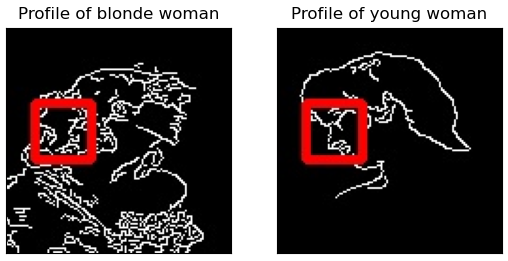
\includegraphics[width=0.45\textwidth]{/home/morita/ros2_ws/output/rectangle0709.png}
            \caption{領域の位置の確認}
            \label{the position of a region}
        \end{figure}
    \end{center}

	

	理由は端点を持つ線から描くほうが人が描いたように見えると直感的に考えたからである
    .
	線の経路の求め方は、ある線の画素から隣に線の画素があるかを探して、移動してを繰り
    返すものとなっている.
	そのため、線を一本に単純化してある方が線をたどるのに容易であるため細線化を行う.
	端点を検出して描くのには2つの理由がある.
	線画を生成する過程で繋がっているはずの線が途切れてしまうというのが一つの理由であ
    る.
	それは平滑化、エッジ抽出、細線化処理を施すからである.
	一方は左上から右下へ走査するラスタスキャンを用いる方法である.

 	\section{ロボットの機構}
	本研究で用いるロボットは3軸のマニピュレータロボットである.
	下の図1のようにアームの先端、姿勢の関節角を$\theta_1, \theta_2, \theta_3$、各リンクの長さ$l_1, l_2, l_3, l_4$とし、逆運動学問題を解く.
	またリンク座標系を定める方法として、DH記法(Denavit-Hartenberg記法)を用いる.

    \begin{center}
        \begin{figure}[h]
            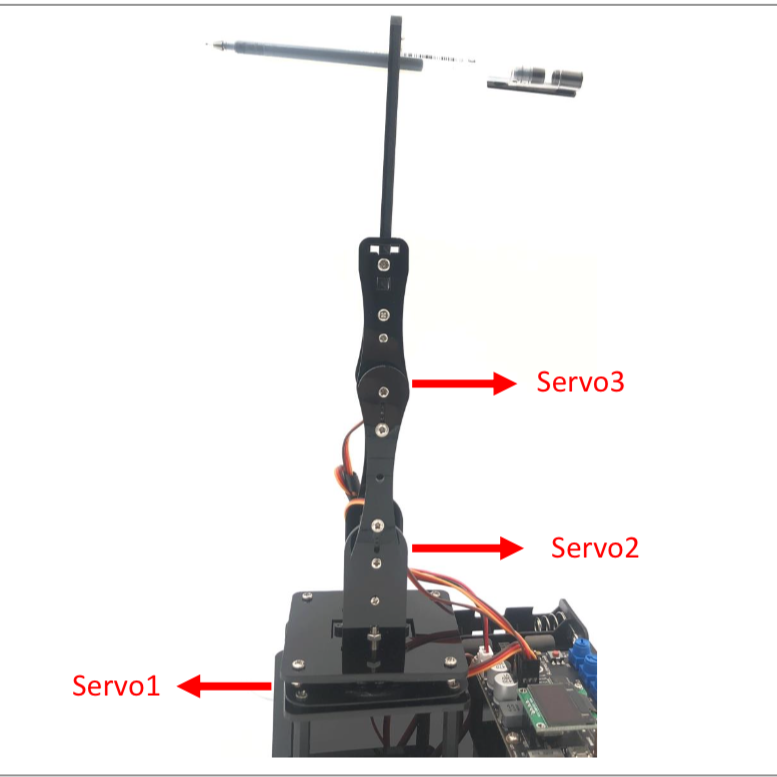
\includegraphics[width=0.45\textwidth]{/home/morita/ros2_ws/Memo/tex/img/IMG_0025.PNG}
            \caption{実機}
            \label{fig:sample-fig}
        \end{figure}
    \end{center}
    
	\section{手先の位置と回転角の関係}
	運動学、逆運動学を用いて、ペン先の位置を各サーボモータの回転角を導出する.
	リンク座標系は以下のように定義し、座標変換を行う.
	
	座標系1から3への座標変換行列は以下のようになる.
    \begin{center}
        \begin{figure}[h]
            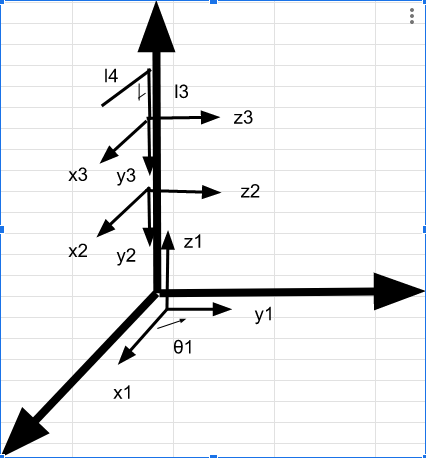
\includegraphics[width=0.45\textwidth]{/home/morita/ros2_ws/Memo/tex/img/link.png}
            \caption{リンク座標系:}
            \label{fig:sample-fig}
        \end{figure}
    \end{center}
$$
	^{0}T_{3}=^{0}T_{1} ^{1}T_{2} ^{2}T_{3} \\
$$
	\begin{equation*}
		\begin{array}{cc}
			=
			\left( 
				\begin{array}{cccc}
					C_1C_{23} & -C_1S_{23} & 0 & l_2C_1S_2 \\
					S_1C_{23} & -S_1S_{23} & 0 & l_2S_1S_2 \\
					-S{23} & -C_{23} & -1 & l_2C_2 + l_1 \\
					0 & 0 & 0 & 1 
				\end{array}
			\right)
		\end{array}
	\end{equation*}
	ただし、
	\begin{equation*}
		\left(
		\begin{split}
			C_{23} = cos\theta_2cos\theta_3-sin\theta_2sin\theta_3\\
			S_{23} = sin\theta_2cos\theta_3+cos\theta_2sin\theta_3	
		\end{split}
		\right)
	\end{equation*}
    また手先ベクトルが以下のように求まる.

	\begin{equation*}
	\begin{array}{cccc}
		&\left(
			\begin{array}{cccc}
				1 & 0 & 0 & l_4\\
				0 & 1 & 0 & 0\\
				0 & 0 & 1 & 0\\
				0 & 0 & 0 & 1
			\end{array}
		\right)
		\left(
			\begin{array}{cccc}
				1 & 0 & 0 & 0\\
				0 & 1 & 0 & -l_3\\
				0 & 0 & 1 & 0\\
				0 & 0 & 0 & 1
			\end{array}
			\right)\\
		&=
		\left(
		\begin{array}{cccc}
			1 & 0 & 0 & l_4\\
			0 & 1 & 0 & -l_3\\
			0 & 0 & 1 & 0\\
			0 & 0 & 0 & 1
		\end{array}
		\right)
	\end{array}
	\end{equation*}
	
	より手先までの座標変換行列$^{0}P_{r}$が以下のように求まる.
	\begin{equation*}
	\begin{array}{cc}
		\left( 
			\begin{array}{cccc}
				C_1C_{23} & -C_1S_{23} & 0 & l_4C_1C_{23}+l_3C_1S_{23}+l_2C_1S_2 \\
				S_1C_{23} & -S_1S_{23} & 0 & l_4S_1C_{23}+l_3S_1S_{23}+l_2S_1S_2 \\
				-S{23} & -C_{23} & -1 & -l_4S_{23}+l_3C_{23}+l_2C_2+l_1 \\
				0 & 0 & 0 & 1 
			\end{array}
		\right)
	\end{array}
	\end{equation*}

	座標変換によって順運動学解が以下のように求まる.
	そしてこの行列から手先の位置x, y, zは以下のように求まる.
	\begin{equation}
		\left\{
			\begin{array}{c}
			\begin{split}
				&  x  =  C_1(l_4C_{23}  +  l_3S_{23}  +  l_2S_2)\quad \\
				&  y  =  S_1(l_4C_{23}  +  l_3S_{23}  +  l_2S_2)\quad \\
				&  z  -  l_1  =  -l_4S_{23}  +  l_3C_{23}  +  l_2C_2\quad \\
			\end{split}
		\end{array}
		\right.
	\end{equation}
	これらの逆運動学を解くと
	\begin{equation}
		\left\{
			\begin{array}{c}
			\begin{split}
				\theta_1  &  =\frac{1}{2}  cos^{-1}\biggl( \frac{x^2-y^2}{x^2+y^2} \biggr) \\
				\theta_2  &  = cos^{-1}\biggl( \frac{x^2+y^2+(z-l1)^2  +  l_2^2-l_3^2-l_4^2}{2l_2\sqrt{x^2+y^2+(z-l_1)^2}} \biggr)\\
				&\qquad\qquad  +  tan^{-1}\biggl( \frac{\sqrt{x^2+y^2}}{z-l1}\biggr) \\
				\theta_3  &  =cos^{-1}\biggl( \frac{x^2+y^2+(z-l1)^2 - l_4^2-l_3^2-l_2^2}{2l_2\sqrt{l_3^2+l_4^2}}\biggr)\\
				&\qquad\qquad + tan^{-1}\biggl( \frac{-l_4}{l_3}\biggr)\\
			\end{split}
			\end{array}
		\right.
	\end{equation}

	\section{手先の到達範囲}
	描画は第一象限で行う.
	この条件と不等式にまとめると以下のようになる.
	\begin{equation*}
		\left\{
			\begin{array}{c}
				\begin{split}
					&  0  \leqq  \theta_1  \leqq  \frac{\pi}{2}  &  \\
					&  x  \geqq  0  \land  y  \geqq  0
				\end{split}
			\end{array}
		\right.
	\end{equation*}

	手先の最大到達点は
	\begin{equation*}
		l_2+l_3  =  65+130  =  195
	\end{equation*}
	また、第一象限に描きたいが、手先が一回転するのは避けたい.
	それはつまり、$  \theta_2  \geqq  0\  (\land)  \  \theta_3  \geqq0$ということである.
	逆運動学解の$\theta_3$を用いると、$  -1  \leqq  cos((\theta_3  -  \alpha)  \leqq  1)$より
	\begin{equation*}
		-2l_2\sqrt{l_3^2+l_4^4}  - (z-l_1)^2  +  (l_4^2  +  l_3^2  +  l_2^2)  \leqq  x^2  +  y^2  \leqq  195
	\end{equation*}
	$$
		(\text{最左辺})  =  116.4208  \cdots
	$$
	よって求めたい手先の範囲は以下のようになる.
	\begin{equation*}
		\therefore\  117  \leqq  x^2  +  y^2  \leqq  195
	\end{equation*}



    
    \section{引用文献の書き方}%===========================
    本文中の引用箇所には,右肩に小括弧をつけて,通し番号を付ける.例えば,文献\cite{工大2005}や,文献\cite{Shibutani2004, Handbook1979, Kikuchi2017, Adrobo2019}のようにする.
    
    引用文献は,英文で記述されているもの(文献\cite{Shibutani2004}など)は英文で書き,本文末尾に引用順にまとめて書く.専門的な書籍(文献\cite{Handbook1979}など)についても引用しても良い.
    Web上の資料を引用する場合,例えばオンラインジャーナルなどの場合は文献\cite{Kikuchi2017}のように,webページの場合は文献\cite{Adrobo2019}のように,それぞれ参考文献として記載して引用する.この時,URLとともに参照日を記載すること.ただし,webページの場合は個人の技術ブログなどのように第3者による十分な審査が行われていないものの引用は行ってはいけない.公的な機関が発行しているページであっても,その永続性の問題から必要最小限に留めることを推奨する.
        
    \section{結\hspace{2zw}言}%===========================
    このスタイルファイル「adrobo\_abst.sty」は,千葉工業大学 未来ロボティクス学科の卒業研究概要として公式に提出可能なように,学科で配布するwordテンプレートとレイアウトなどの体裁を合わせたものである.
    ただし,絶対的な出来上がりのレベルを保証するものではないため,執筆を進める上で不具合などが生じた場合は,直ちに製作者に通知をすることが望まれる.
    また,使用者によるスタイルファイルの微調整などに関しては,自己責任の範囲において自由に行って良い.
    
    \vspace{5truemm}
    {\footnotesize
        \begin{thebibliography}{99}
            
            \bibitem{工大2005}
            工大太郎: ``ロボットのしくみ'', 
            日本機械学会論文誌A, 
            Vol.~108, No.~1034 (2005), pp.~1--2.
            
            \bibitem{Shibutani2004}
            Y. Shibutani: ``Heinrich's Law Resulted Pattern Dynamics --Part2--'',
            Proceedings of the 79th Kansai Branch Regular Meeting of the Japan Society of Mechanical Engineers,  
            No.~04--05 (2004), pp.~205--206.
            
            \bibitem{Handbook1979}
            The Japan Society of Mechanical Engineers ed.: ``JSME Date Handbook: Heat Transfer'', 
            (1979), p.~123, The Japan Society of Mechanical Engineers.
            
            \bibitem{Kikuchi2017}
            K. Kikuchi, M. Miura, K. Shibata, J. Yamamura: ``Soft Landing Condition for Stair-climbing Robot with Hopping Mechanism'', 
            Journal of JSDE, Vol.~53, No.~8 (2018), pp.~605--614, \url{https://doi.org/10.14953/jjsde.2017.2774}.
            
            \bibitem{Adrobo2019}
            千葉工業大学 未来ロボティクス学科 学科概要: 
            \url{http://www.robotics.it-chiba.ac.jp/ja/subject/index.html}, 
            (参照日 2023年1月29日). 
            
        \end{thebibliography}
    }
    \normalsize
    
\end{document}
